\documentclass[../main.tex]{subfiles}

\section{Variables}
\begin{document}
When a program is running, there is a lot of data manipulation going on in the
processor and memory of it. While some data are constant that remain the same
value while programming is running, others are changable, and they are usually
refered as `variable'. In computer, a variable is a memory location that is
associated with a symbolic name.

An analogy in math is function. For a linear function such as:\[f(x) = x + 1\]

In the expression above, \(x\) is considered as a variable: you can assign any
numerical value to it, and that expression will just evaluate what ever you assign
to \(x\). Of course, you can also assign the result of the function above to
another variable, say \(y\), and the expression will look like this:
\[y = x + 1\]

If we have a variable \(x\) and the valued stored in it is 20, then we will get
21 if we plug \(x\) in the expression above. If we have another variable \(y\), we
can assign 21 to it and \(y\) will have value 21.

However, you should also notice that you can only plug in a numerical value to
\(x\). It does not make any sense to evaluate the sum of ``banana'' and 1. This
is a very important lesson for us: sometimes a function can only accept certain
kind of input, and that kind is usually called ``type'' in computer science. In
this case, our function above can only accept numerical inputs. In another word,
\(x\) must be a number.

In programming, variables can be created by programmer or program, depends on
the job that the programm wants to perform. Variables must be \emph{declared}
before they can be \emph{referred} or \emph{assigned}. The \emph{declaration} of
a variable is the creation of that variable: programmer ask the operating system
to allocate a chunk of memory to store some value. The \emph{reference} of a
variable is to obtain or use the value stored in that variable. The \emph{assignment}
of variable is to assign a new value to a particular variable. Remember, you must
declare the variable first before you can either refer to it or assign value
to it.

% Now introduce the variable in C#.
\subsection{Variable Declaration in C$\sharp$}
C$\sharp$ is a statically-typed programming langauge, meaning that every variable
you declared in C$\sharp$ programming language must have a type.

\subsection{Variable Naming}
When your program is running, the program accesses variables that you allocated
by using their memory addresses instead of those symbolic names that you put in
code. You may wonder: if the program does not necessarily need the name of
variable, why do we care about the naming of it?

The truth is, your program is not only just for solving a programming problem.
If you are working with a large programming team, your code is very likely to
be read by tens, if not hunderds or thousands, of people, and people need to
understand what your code is doing even when you left the team. Having good
naming of variables make your code self-documented, thus brings good code and
maintainable program.

Compare the following pairs of naming:
\begin{itemize}
    \item An integer variable for age: age and x
    \item A string variable for user input: input and s
    \item A double variable for balance of savings account: savingBalance and b1
\end{itemize}
By comparing the naming choices above, you probably have noticed that good
naming choice for variables can be very helpful in programming.

\subsection{Primitive Type and Reference Type}
Besides that values have all kinds of types, the storage of those values has
type as well. There are two commonly used storage type in today's programming
language: primitive type and reference type.

A primitive type (or variable type) is type of storage that the value of the
variable is directly stored at where it is allocated. Imagine that you have a
group of boxes, items are stored right instead of these boxes. For example, if
we write a program like this:

\begin{minted}{csharp}
    using System;
    public class Program
    {
        public static void Main (string [] args)
        {
            double price = 14.99;
            int unit = 5;
            float taxRate = 0.01f;
            double sum = price * unit * (1 + taxRate);
            Console.WriteLine ("Unit price: " + price);
            Console.WriteLine ("Purchases: " + unit);
            Console.WriteLine ("Tax Rate: " + taxRate);
            Console.WriteLine ("Total Cost: " + sum);
        }
    }
\end{minted}

In this case, variable \texttt{price}, \texttt{unit}, \texttt{taxRate}, \texttt{sum}
are primitive type and the value are stored in the memory box that they reside
in. If we draw a memory diagram of those variables that we declared, it would
look like this:

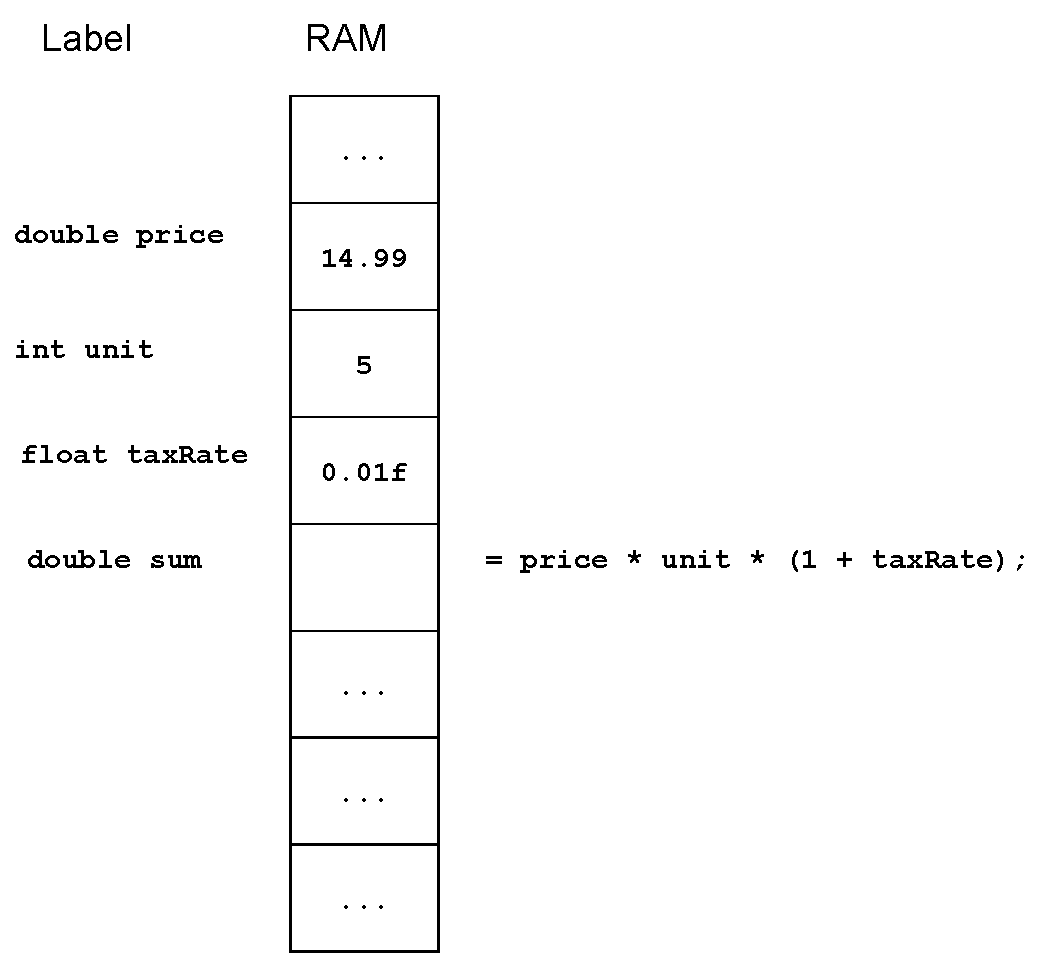
\includegraphics[scale = 0.5]{type/img/mmap-primitive.pdf}

In this case, 

Reference type (also called as \emph{pointer type}) is a little bit different.
Inside of directly putting items inside the box, reference type will put the
address of the item inside the box. When you need that value, you open the box
first, and notice that there is only the address of values that you want. Then
you follow the address and find the value.

Why do we need both of them? Think about this way: each memory address has
limited capacity for storing values. However, sometimes there are values that
are so huge that would take many many addresses of spaces to store. In this case,
it would be unrealistic to squeeze all those values in one little address. We
need to split them and use a pointer to find out the first item of those values.
Based on the type of that pointer, we can also easily find the other values
of the variable.

Another advantage of using reference type is that using reference type can save
time on memory reallocation. If you have a chunk of data of 3 gigabyte in memory,
it would be time wasting to move this much data around the memory avery time we
use it. However, with reference type, we can simply use a different reference to
achive the `movement' of data.

\end{document}
